\documentclass[paper=letter,fontsize=11pt,DIV=14]{scrartcl}

\KOMAoptions{captions=tableheading,bibliography=totoc}

\usepackage[cleanlook,british]{isodate}
\usepackage{amsmath,amsthm,amssymb}
\usepackage[plextt,lucida]{mycommon}
\usepackage{csquotes}
\usepackage{booktabs,tabularx}
\usepackage{caption,subcaption}
\usepackage[export]{adjustbox}
\usepackage{graphicx}
\usepackage[inline]{enumitem}
\usepackage{float}

\title{Workflow for ``Understanding Developers' Addition and Removal of Type Annotations'' (IRB 23988)}
\author{}
\date{}

\usepackage{nameref}
\usepackage[pdfa]{hyperref}
\usepackage{hyperxmp}
\usepackage[nameinlink]{cleveref}

\newcommand{\flowref}[1]{\hyperref[{#1}]{\nameref*{#1} flow (\S \ref*{#1})}}

\begin{document}

\maketitle

At any time during the monitoring period, a person may submit an opt out command as a commit comment on a commit in any monitored project (at which point the \flowref{opts-out} is followed).
They may likewise request removal of their data (and the \flowref{removal-requested} is followed).

\paragraph*{Note on Conventions and Assumptions}
\label{note-on-conventions-and-assumptions}

In this document, comments made by our bot are marked with \texttt{(BOT\ COMMENT)} for clarity.
Upon deployment, these comments will not include this phrase, as GitHub marks bot actions automatically.

Additionally, we assume that we are dealing with projects which have agreed to participate in this project.

Finally, some small details (exact location of study website, the name of the bot) have not yet been determined.
In particular, in this document, the bot referred to as \texttt{@UNLPALBOTACCT} will be given a slightly different name.

\section{Start}
\label{start}

A commit which adds or removes a type annotation has been detected (see \Cref{fig:commit-detected}).

\begin{figure}[H]
\centering
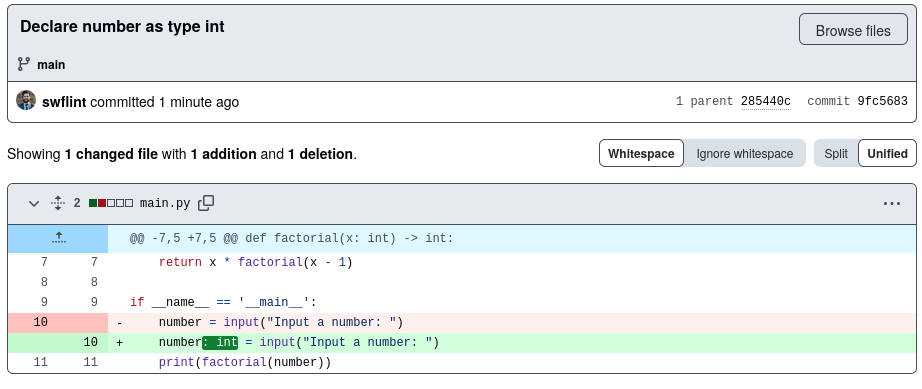
\includegraphics[height=6cm,frame]{./commit-detected.png}
\caption{Commit with addition or removal of type annotation detected}
\label{fig:commit-detected}
\end{figure}

Then,
\begin{itemize}[noitemsep]
\item If the committer is on the opt-out list, do nothing.
\item If the committer is not listed, go to the \flowref{not-listed}
\item If the committer has consented, go to the \flowref{send-survey}
\item If the committer is listed as having been contacted, but has not consented, STOP.
\end{itemize}

\section{Participant Not Listed}
\label{not-listed}

Place committer on list of contacted committers and send request for consent message (see \Cref{fig:request-consent}).

\begin{figure}[H]
\centering
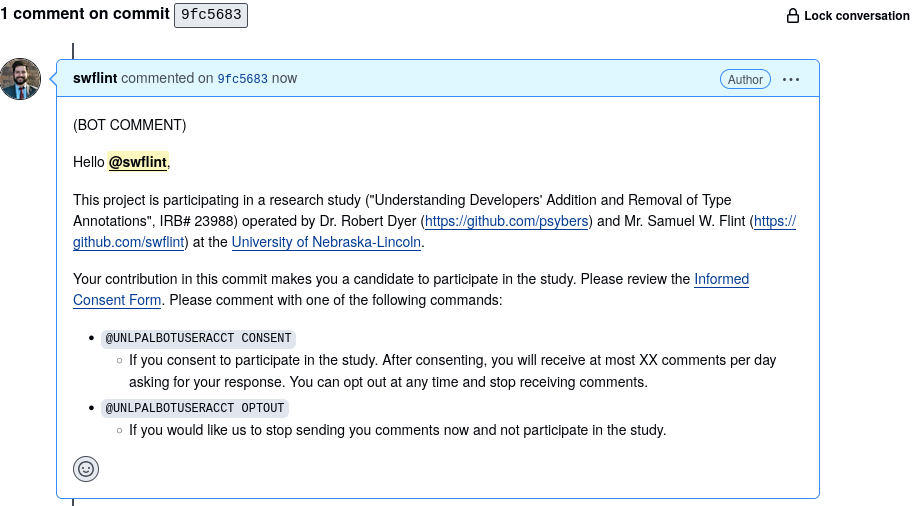
\includegraphics[keepaspectratio,width=\linewidth,height=8cm,frame]{./request-consent.png}
\caption{Request for consent}
\label{fig:request-consent}
\end{figure}

Then,
\begin{itemize}[noitemsep]
\item If the committer ignores the message, do nothing.
\item If the committer responds with \texttt{@UNLPALBOTACCT\ CONSENT} (see \Cref{fig:consented}), record consent information, and go to the \flowref{send-survey}.
  \begin{figure}[H]
    \centering
    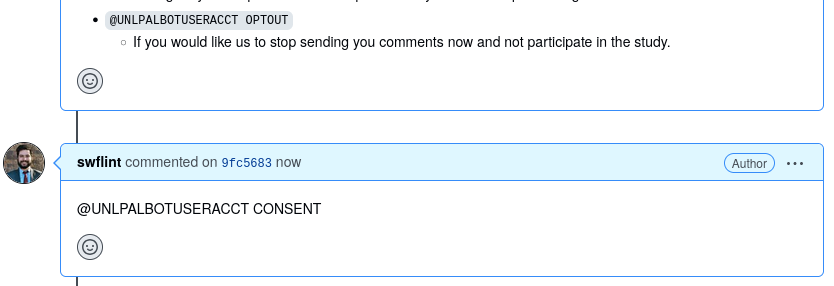
\includegraphics[height=4cm,frame]{./consented.png}
    \caption{Participant responds with consent message}
    \label{fig:consented}
  \end{figure}

\item If the committer responds with \texttt{@UNLPALBOTACCT\ OPTOUT} (see \Cref{fig:optout}) go to the \flowref{opts-out}.
  \begin{figure}[h]
    \centering
    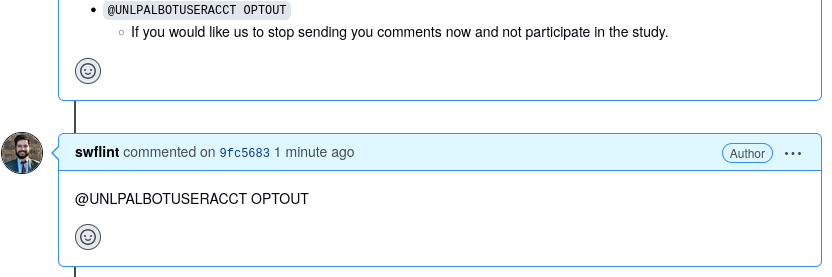
\includegraphics[width=\linewidth,frame]{./optsout.png}
    \caption{Participant has requested to opt-out (Note: this can happen on any commit made to a monitored project)}
    \label{fig:optout}
  \end{figure}
\end{itemize}

\section{Participant Consents}\label{send-survey}

Committer is not on opt-out list, and has consented to participate in the study.

If this is the first time a participant is surveyed, we will send a one-question general survey, as shown in \Cref{fig:general-survey}.
If they have been surveyed before, go to the \flowref{send-primary-survey}.

\begin{figure}[h]
\centering
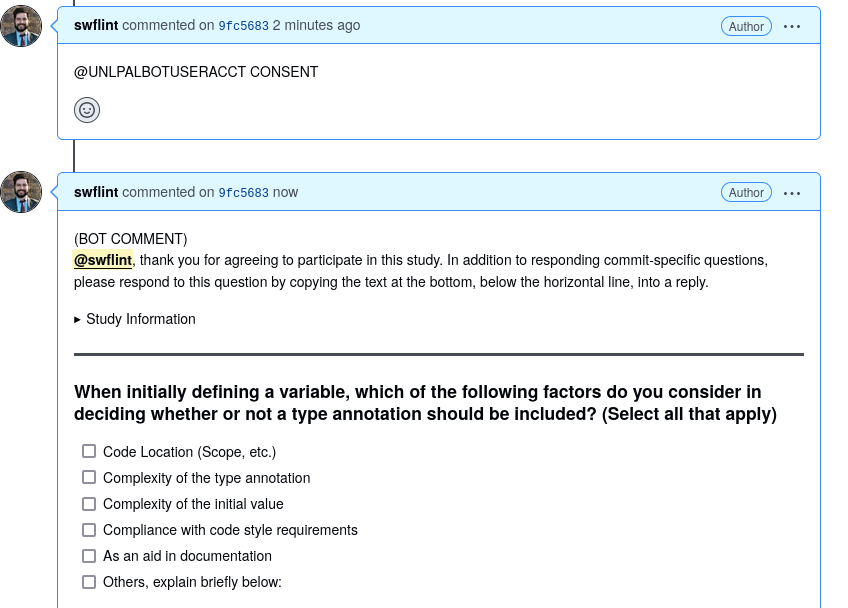
\includegraphics[width=\linewidth,frame]{./presurvey.png}
\caption{General, single-question pre-survey}
\label{fig:general-survey}
\end{figure}

\section{Send Primary Survey}
\label{send-primary-survey}

Based on the last time the participant was asked to respond, we will send a short survey, ensuring that participants are not contacted more than one time a 24-hour period (see \Cref{fig:survey}).
The survey will be submitted on the line which introduces the type change.

\begin{figure}[h]
\centering
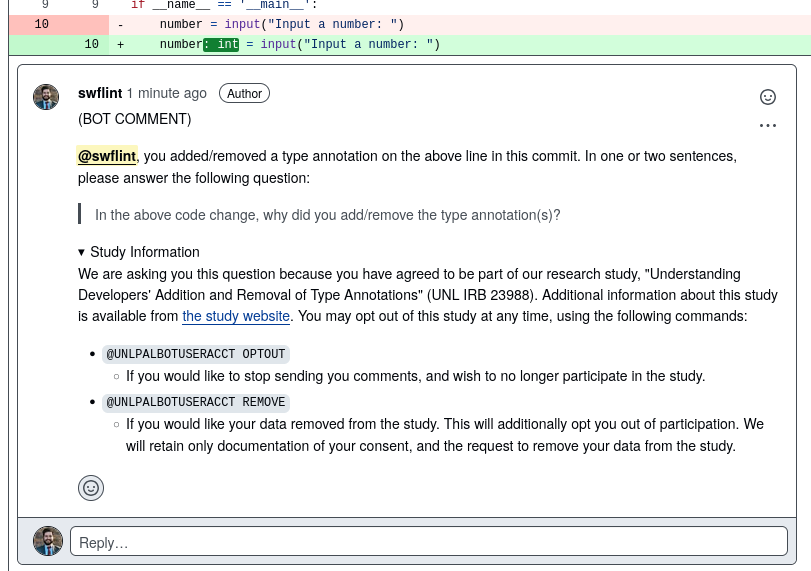
\includegraphics[width=\linewidth,frame]{./survey-sent.png}
\caption{Participant sent survey}\label{fig:survey}
\end{figure}

\begin{itemize}[noitemsep]
\item If the participant responds to the survey, record the response, and show an acknowledgment (see \Cref{fig:survey-response}).
  \begin{figure}[h]
    \centering
    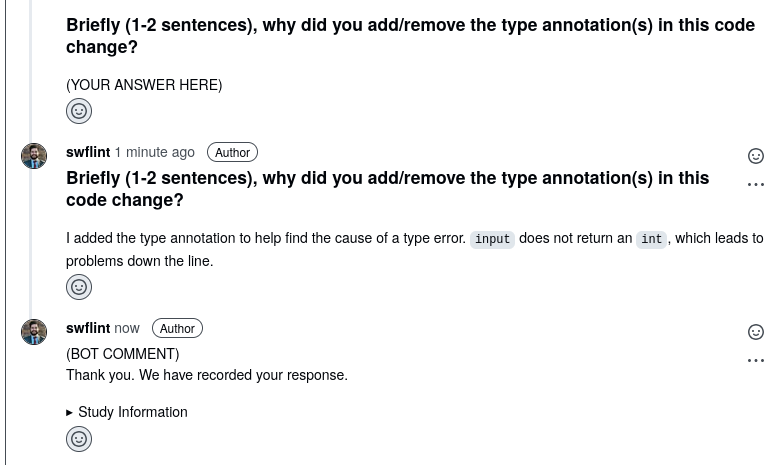
\includegraphics[width=\linewidth,frame]{./survey-response.png}
    \caption{Participant responds to survey}
    \label{fig:survey-response}
  \end{figure}

\item If the participant submits \texttt{@UNLPALBOTACCT\ OPTOUT} (see \Cref{fig:optout}), go to the \flowref{opts-out}.
\item If the participant submits \texttt{@UNLPALBOTACCT\ REMOVE} (see \Cref{fig:removal-request}), go to the \flowref{removal-requested}.
  \begin{figure}[h]
    \centering
    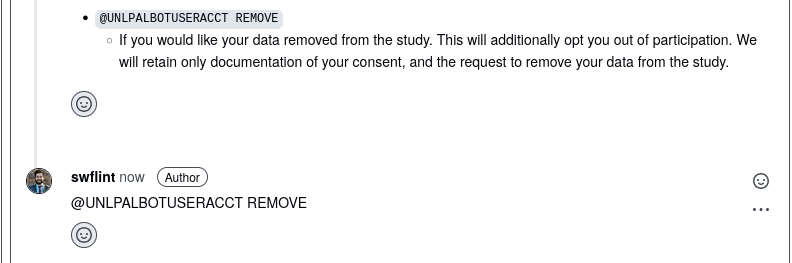
\includegraphics[width=\linewidth,frame]{./removal-request.png}
    \caption{Participant requests removal of data}
    \label{fig:removal-request}
  \end{figure}

\end{itemize}

\section{Participant Opts Out}\label{opts-out}

The participant/committer is placed on the opt-out list, and sent an acknowledgment (see \Cref{fig:opt-out-removal-ack}).

\begin{figure}[h]
\centering
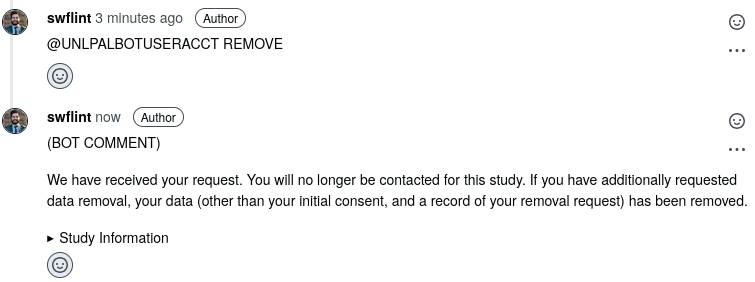
\includegraphics[width=\linewidth,frame]{./acknowledgment-removal.png}
\caption{Acknowledgment of opt-out or data removal request}
\label{fig:opt-out-removal-ack}
\end{figure}

\section{Participant Requests Removal Of Data}\label{removal-requested}

A participant has submitted the command \texttt{@UNLPALBOTACCT\ REMOVE}.
A record of the removal request, and opt-out is made.
Data other than removal request, opt-out, and initial consent is removed from the server.
We then send an acknowledgment of the request (see \Cref{fig:opt-out-removal-ack}).



\end{document}

%%% Local Variables:
%%% mode: LaTeX
%%% TeX-master: t
%%% End:
